% !TEX encoding = UTF-8
% !TEX TS-program = pdflatex
% !TEX root = ../tesi.tex

%**************************************************************
\chapter{Analisi dei requisiti}
\label{cap:analisi-requisiti}
%**************************************************************

\intro{In questo capitolo viene esposta l'analisi dei requisiti effettutata durante lo stage, nella quale si descrivono le funzionalità e i requisiti identificati.}\\
\section{Analisi del prodotto}
	\subsection{Descrizione del prodotto}
		\subsubsection{Contesto}
			Il prodotto sarà utilizzato internamente dall'azienda Euronovate per il monitoraggio della validità delle \gloxy{S.L.A.}, e per un'analisi statistica delle segnalazioni aperte da \gloxy{Customers}.
		\subsubsection{Funzionalità} 
			Il prodotto deve interfacciarsi con il software \gloxy{Redmine}, già utilizzato dall'azienda per la raccolta delle segnalazioni da parte dei clienti, per l'ottenimento dei dati, i quali poi dovranno essere analizzati e in caso di violazioni, dovranno essere predisposti diversi canali di notifica, per la segnalazione della violazione.\\
			Infine, i dati saranno salvati in una base di dati, ed esposti tramite un \gloxy{API} con un fine di analisi statistica di essi.
		\subsection{Analisi della struttura} 
			Il prodotto prevede principalmente 4 sistemi: l'\gloxy{API} di pubblicazione, il sistema di ottenimento dei dati, il sistema di analisi, ed infine il sistema di notifica.
		\subsubsection{Sistema ottenimento dati} 
			Il sistema ottenimento dati sistema è responsabile dell'ottenimento dei dati da \gloxy{Redmine}, quali \gloxy{Customers} e \gloxy{Ticket} aperti da clienti. \\
			Questo sistema deve autenticarsi su \gloxy{Redmine}, ottenere i dati, e manipolarli in modo da prevedere una loro semplice integrazione con gli altri servizi.
			Tale download dei dati verrà effettuato in batch, quindi periodicamente l'engine andrà a scaricarsi gli aggiornamenti. \\
			deve infine esser possibile migrare a un servizio di segnalazione esterno diverso da \gloxy{Redmine}, senza andare a modificare gli altri sistemi.
		\subsubsection{Sistema analisi dati}
			Il sistema analisi dati è responsabile dell'analisi dei dati e delle \gloxy{S.L.A.}. definite con i vari clienti. \\
			È quindi stato necessario predisporre un sistema di configurazione delle \gloxy{S.L.A.}. dei clienti dinamico, che non richieda il riavvio del sistema. \\
			Inoltre, una volta analizzato dati e \gloxy{S.L.A.}., è responsabile  della comunicazione con il servizio di notifica per la segnalazione di violazioni.
		\subsubsection{Sistema di notifica}
			Il sistema di notifica sarà responsabile della notifica delle violazioni ai responsabili.\\
			È stato quindi necessario predisporre vari mezzi di notifica, configurabili dinamicamente, che permettano la segnalazione a chi di dovere della potenziale violazione delle \gloxy{S.L.A.}., in base a quanto grave essa sia.
		\subsubsection{Sistema di pubblicazione}
			Il sistema di pubblicazione è responsabile della pubblicazione dei dati gestiti verso l'esterno.\\
			È quindi stato necessario predisporre un \gloxy{API} tramite la quale gli interessati potranno accedere alle informazioni gestite dall'engine, quali issue, customer e violazioni. \\
			È desiderabile permettere di definire se il risultato lo si vuole dalla base di dati attuale (e quindi aggiornato all'ultimo update), o lo si vuole esattamente fino a quel momento, e quindi richiedendo un aggiornamento immediato da \gloxy{Redmine}.
		






\section{Casi d'uso}

In questa sezione sono elencati i casi d'uso rilevati nell'analisi dei requisiti del progetto.\\
Per lo studio dei casi di utilizzo del prodotto sono stati creati dei diagrammi.\\
I diagrammi dei casi d'uso (in inglese \emph{Use Case Diagram}) sono diagrammi di tipo \gls{uml} dedicati alla descrizione delle funzioni o servizi offerti da un sistema, così come sono percepiti e utilizzati dagli attori che interagiscono col sistema stesso.
Essendo il progetto incentrato sullo sviluppo dell'engine, le interazioni da parte dell'utilizzatore sono ovviamente ridotte allo stretto necessario. Per questo motivo i diagrammi d'uso risultano semplici e in numero ridotto.\\

\noindent Ogni caso d’uso ha un codice gerarchico ed univoco che lo identifica, nella forma:
\begin{center}
	\textbf{UC<CodicePadre>.<CodiceFiglio>}
\end{center}
Il codice progressivo può includere diversi livelli di gerarchia separati da un punto.

\subsection{Attori}
Gli attori individuati dopo un’attenta analisi sono i seguenti:


\begin{center}
	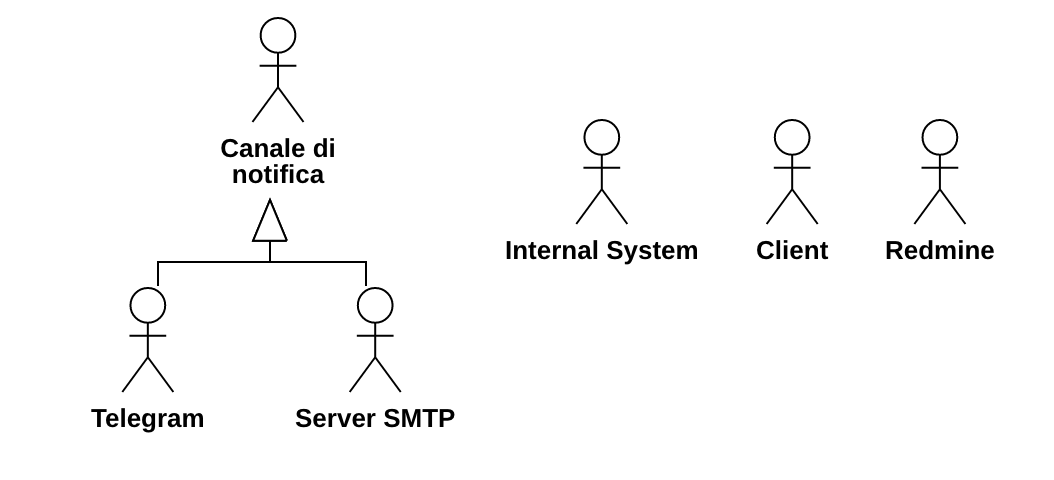
\includegraphics[keepaspectratio = true, width=15cm]{immagini/actors.png}
	\captionof{figure}{Attori individuati}
\end{center}

\subsubsection{Redmine}
\gloxy{Redmine} rappresenta il sistema di gestione di progetto e tracciamento delle segnalazioni utilizzato dall'azienda.
\subsubsection{Telegram}
\gloxy{Telegram} rappresenta uno dei canali di notifica identificati per la segnalazione delle violazioni.
\subsubsection{Server SMTP}
L'email rappresenta uno dei canali di notifica identificati per la segnalazione delle violazioni.
\subsubsection{Client}
Con Client si vuole identificare qualsiasi attore capace di consumare l'\gloxy{API}  (come un Front-end, un altro server ...).
\subsubsection{Internal System}
Con Internal System si vuole identificare la piattaforma ENTicketEngine stessa.


\subsection{Sistema di ottenimento dati}
Gli use case identificati per questo sistema possono essere riassunti mediante il seguente diagramma UML:
\begin{center}
	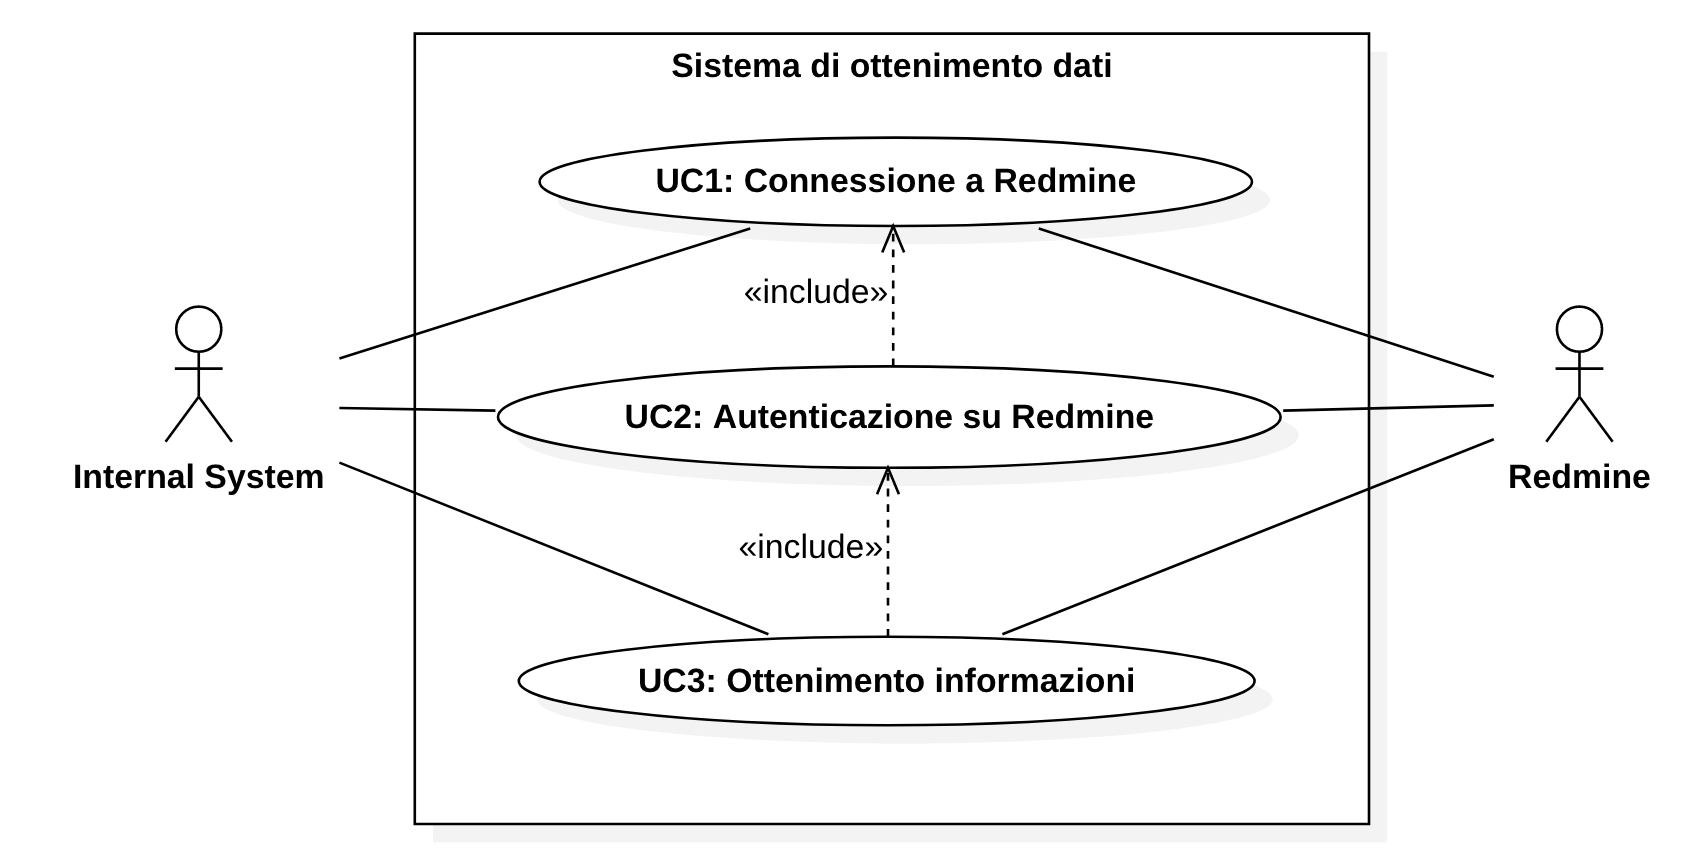
\includegraphics[keepaspectratio = true, width=15cm]{immagini/uc/1.png}
	\captionof{figure}{Use Case sistema di ottenimento dati}
\end{center}
\subsubsection{UC1 - Connessione a Redmine}
\begin{itemize}
	\item \textbf{attore primario}: Internal System;
	\item \textbf{attore secondario}: \gloxy{Redmine};
	\item \textbf{descrizione}: l'engine desidera connettersi a \gloxy{Redmine} per accedere alle sue funzionalità;
	\item \textbf{precondizione}: l'engine non ha ancora effettuato la connessione a \gloxy{Redmine};
	\item \textbf{postcondizione}: l'engine ha una connessione a \gloxy{Redmine} stabilita;
	\item \textbf{scenario principale}: 
	\begin{enumerate}
		\item Il sistema invia una richiesta di connessione a \gloxy{Redmine}.
	\end{enumerate}
\end{itemize}

\subsubsection{UC2 - Autenticazione su Redmine}
\begin{itemize}
	\item \textbf{attore primario}: Internal System;
	\item \textbf{attore secondario}: \gloxy{Redmine};
	\item \textbf{descrizione}: l'engine vuole autenticarsi presso \gloxy{Redmine} così da poter accedere alle sue funzionalità;
	\item \textbf{precondizione}: l'engine ha una connessione disponibile verso il server \gloxy{Redmine};
	\item \textbf{postcondizione}: il sistema è autenticato presso \gloxy{Redmine} e ha accesso ai dati;
	\item \textbf{scenario principale}: 
	\begin{enumerate}
		\item il sistema invia una richiesta a \gloxy{Redmine} contenente la propria \gloxy{API}  key per l'autenticazione.
	\end{enumerate}
\end{itemize}
\subsubsection{UC3 - Ottenimento informazioni da Redmine}
\begin{center}
	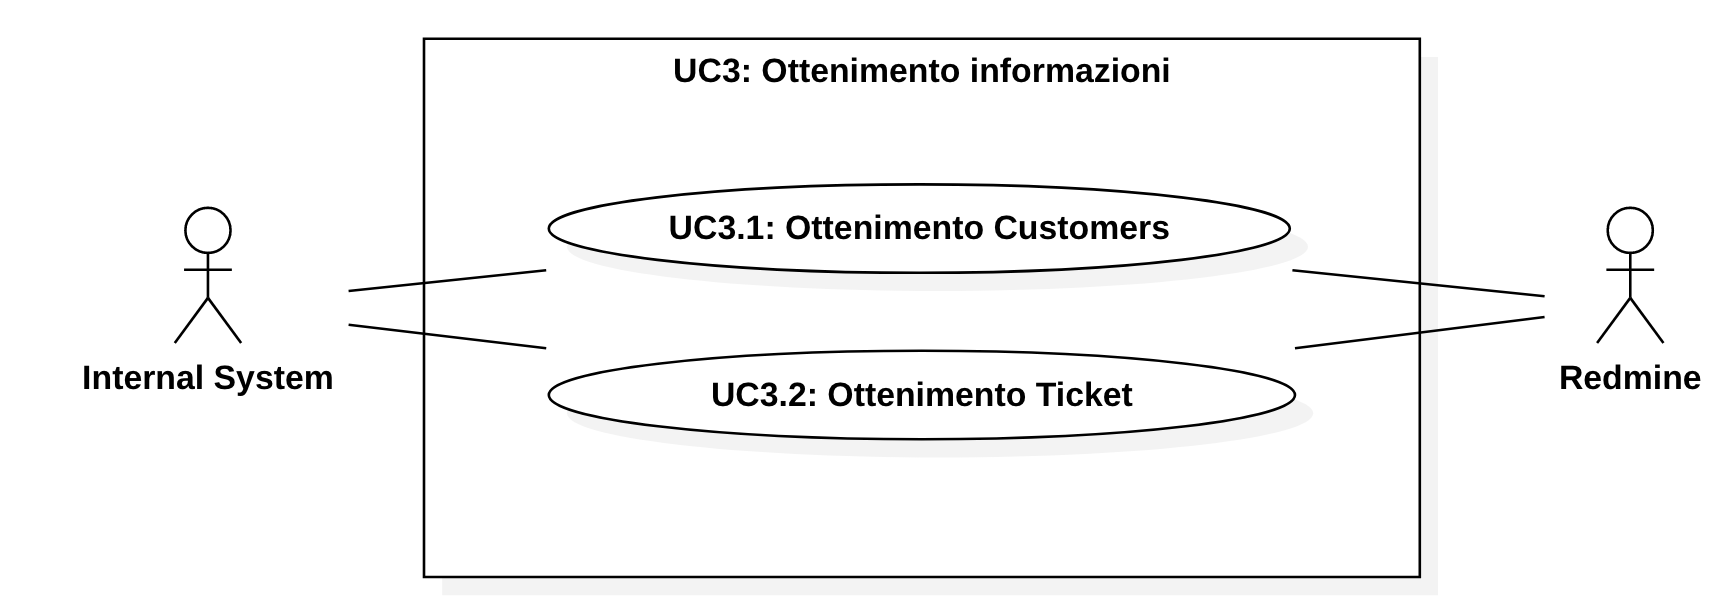
\includegraphics[keepaspectratio = true, width=15cm]{immagini/uc/2.png}
	\captionof{figure}{Sottocasi d'uso UC3}
\end{center}
\begin{itemize}
	\item \textbf{attore primario}: Internal System;
	\item \textbf{attore secondario}: \gloxy{Redmine};
	\item \textbf{descrizione}: l'engine vuole ottenere le informazioni da \gloxy{Redmine};
	\item \textbf{precondizione}: l'engine ha una connessione disponibile verso il server \gloxy{Redmine} ed è autenticato presso esso;
	\item \textbf{postcondizione}: il sistema ottiene i dati richiesti da \gloxy{Redmine};
	\item \textbf{scenario principale}: 
	\begin{enumerate}
		\item il sistema invia una richiesta a \gloxy{Redmine} verso l'endpoint stabilito contenente la propria \gloxy{API key} usata l'autenticazione;
		\item il sistema riceve i dati richiesti.
	\end{enumerate}
\end{itemize}
\paragraph{UC3.1 - Ottenimento Customer}
\begin{itemize}
	\item \textbf{attore primario}: Internal System;
	\item \textbf{attore secondario}: \gloxy{Redmine};
	\item \textbf{descrizione}: l'engine vuole ottenere i \gloxy{Customers}  da \gloxy{Redmine};
	\item \textbf{precondizione}: l'engine ha una connessione disponibile verso il server \gloxy{Redmine} ed è autenticato presso di esso;
	\item \textbf{postcondizione}: il sistema ottiene i \gloxy{Customers}  da \gloxy{Redmine};
	\item \textbf{scenario principale}: 
	\begin{enumerate}
		\item il sistema invia una richiesta a \gloxy{Redmine} verso l'endpoint stabilito contenente la propria \gloxy{API key} usata l'autenticazione;
		\item il sistema riceve la lista dei \gloxy{Customers}  richiesti.
	\end{enumerate}
\end{itemize}
\paragraph{UC3.2 - Ottenimento Ticket}
\begin{itemize}
	\item \textbf{attore primario}: Internal System;
	\item \textbf{attore secondario}: \gloxy{Redmine};
	\item \textbf{descrizione}: l'engine vuole ottenere i Ticket da \gloxy{Redmine};
	\item \textbf{precondizione}: l'engine ha una connessione disponibile verso il server \gloxy{Redmine} ed è autenticato presso di esso;
	\item \textbf{postcondizione}: il sistema ottiene i ticket da \gloxy{Redmine};
	\item \textbf{scenario principale}: 
	\begin{enumerate}
		\item il sistema invia una richiesta a \gloxy{Redmine} verso l'endpoint stabilito contenente la propria \gloxy{API key} usata l'autenticazione;
		\item il sistema riceve la lista dei Ticket richiesti.
	\end{enumerate}
\end{itemize}
\subsection{Sistema di analisi dati}
Gli use case identificati per questo sistema possono essere riassunti mediale il seguente diagramma UML:
\begin{center}
	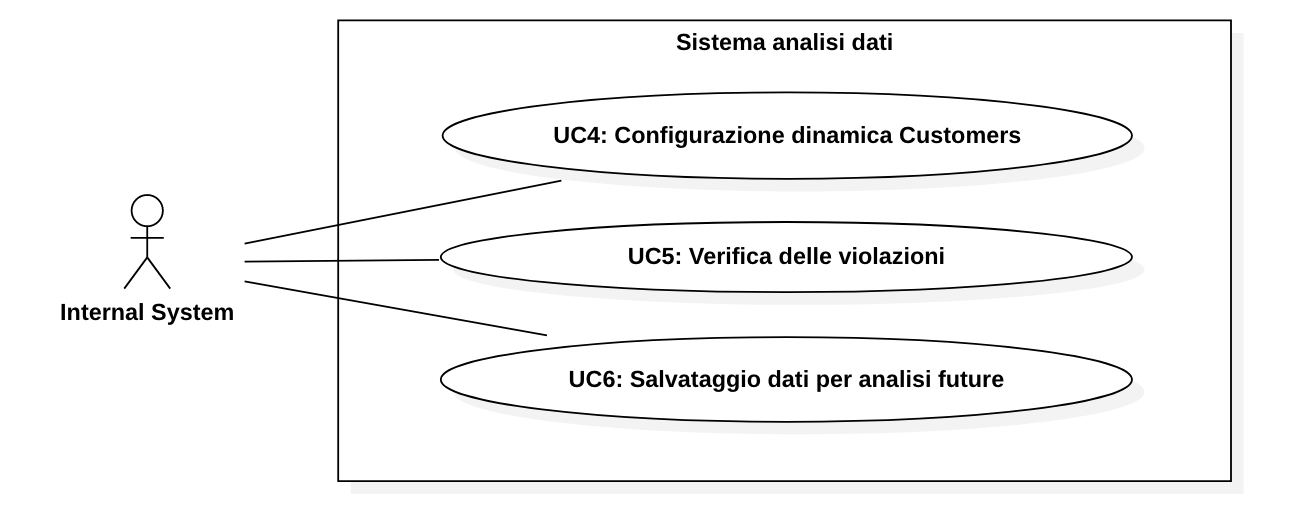
\includegraphics[keepaspectratio = true, width=15cm]{immagini/uc/3.png}
		\captionof{figure}{Use Case sistema analisi dati}
\end{center}
\subsubsection{UC4 - Configurazione dinamica dei Customers}
\begin{center}
	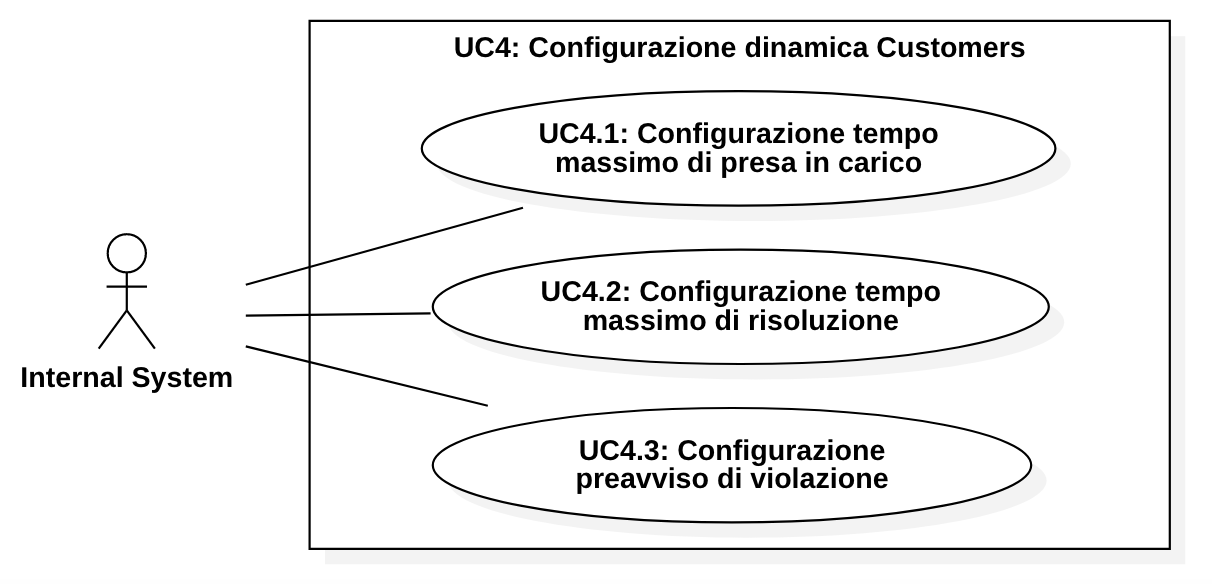
\includegraphics[keepaspectratio = true, width=15cm]{immagini/uc/4.png}
		\captionof{figure}{Sottocasi d'uso UC4}
\end{center}
\begin{itemize}
	\item \textbf{attore primario}: Internal System;
	\item \textbf{descrizione}: il sistema deve disporre di un metodo di configurazione dinamica dei vati \gloxy{Customers} ;
	\item \textbf{precondizione}: il sistema è in uno stato pronto per leggere la configurazione;
	\item \textbf{postcondizione}: il sistema ha letto la configurazione correttamente;
	\item \textbf{scenario principale}: 
	\begin{enumerate}
		\item il sistema apre un file di configurazione e legge le informazioni necessarie.
	\end{enumerate}
\end{itemize}
\paragraph{UC4.1 - Configurazione del tempo massimo di presa in carico di un Ticket}
\begin{itemize}
	\item \textbf{attore primario}: Internal System;
	\item \textbf{descrizione}: il sistema deve disporre di un modo per configurare il tempo massimo di presa in carico di un ticket per ogni \gloxy{Customer}; 
	\item \textbf{precondizione}: il sistema è pronto per leggere la propria configurazione;
	\item \textbf{postcondizione}: il sistema ha letto la configurazione correttamente per ogni \gloxy{Customer}; 
	\item \textbf{scenario principale}: 
	\begin{enumerate}
		\item il sistema legge la configurazione e viene a conoscenza del tempo massimo di presa in carico di un Ticket per ogni suo Customer.
	\end{enumerate}
\end{itemize}
\paragraph{UC4.2 - Configurazione del tempo massimo di presa in risoluzione di un Ticket}
\begin{itemize}
	\item \textbf{attore primario}: Internal System;
	\item \textbf{descrizione}: il sistema deve disporre di un modo per configurare il tempo massimo di risoluzione di un ticket per ogni \gloxy{Customer}; 
	\item \textbf{precondizione}: il sistema è pronto per leggere la propria configurazione;
	\item \textbf{postcondizione}: il sistema ha letto la configurazione correttamente per ogni \gloxy{Customer}; 
	\item \textbf{scenario principale}: 
	\begin{enumerate}
		\item il sistema legge la configurazione e viene a conoscenza del tempo massimo di risoluzione di un Ticket per ogni suo Customer.
	\end{enumerate}
\end{itemize}
\paragraph{UC4.3 - Configurazione preavviso di violazione delle S.L.A.}
\begin{itemize}
	\item \textbf{attore primario}: Internal System;
	\item \textbf{descrizione}: il sistema deve disporre di un modo per configurare il preavviso di notifica che si vuole avere prima di violare una \gloxy{S.L.A.};
	\item \textbf{precondizione}: il sistema è pronto per leggere la propria configurazione;
	\item \textbf{postcondizione}: il sistema ha letto la configurazione correttamente per ogni \gloxy{Customer}; 
	\item \textbf{scenario principale}: 
	\begin{enumerate}
		\item il sistema legge la configurazione e viene a conoscenza del preavviso di notifica desiderato per ogni suo Customer.
	\end{enumerate}
\end{itemize}

\subsubsection{UC5 - Verifica delle violazioni}
\begin{itemize}
	\item \textbf{attore primario}: Internal System;
	\item \textbf{descrizione}: il sistema deve poter analizzare i dati basandoli sulle configurazioni;
	\item \textbf{precondizione}: il sistema è in uno stato pronto per leggere la configurazione;
	\item \textbf{postcondizione}: il sistema ha letto la configurazione correttamente;
	\item \textbf{scenario principale}: 
	\begin{enumerate}
		\item il sistema apre un file di configurazione e legge le informazioni necessarie.
	\end{enumerate}
\end{itemize}
\subsubsection{UC6 - Salvataggio dati per analisi future}
\begin{itemize}
	\item \textbf{attore primario}: Internal System;
	\item \textbf{descrizione}: il sistema deve poter salvare i dati per analisi future;
	\item \textbf{precondizione}: il sistema ha ricevuto dei dati non ancora presenti nella base di dati;
	\item \textbf{postcondizione}: il sistema ha una base di dati aggiornata con i dati appena ricevuti;
	\item \textbf{scenario principale}: 
	\begin{enumerate}
		\item il sistema riceve dei nuovi dati (e.g. da \gloxy{Redmine});
		\item il sistema salva i dati mancanti nella base di dati.
	\end{enumerate}
\end{itemize}
\subsection{Sistema di notifica}
Gli use case identificati per questo sistema possono essere riassunti mediale il seguente diagramma UML:
\begin{center}
	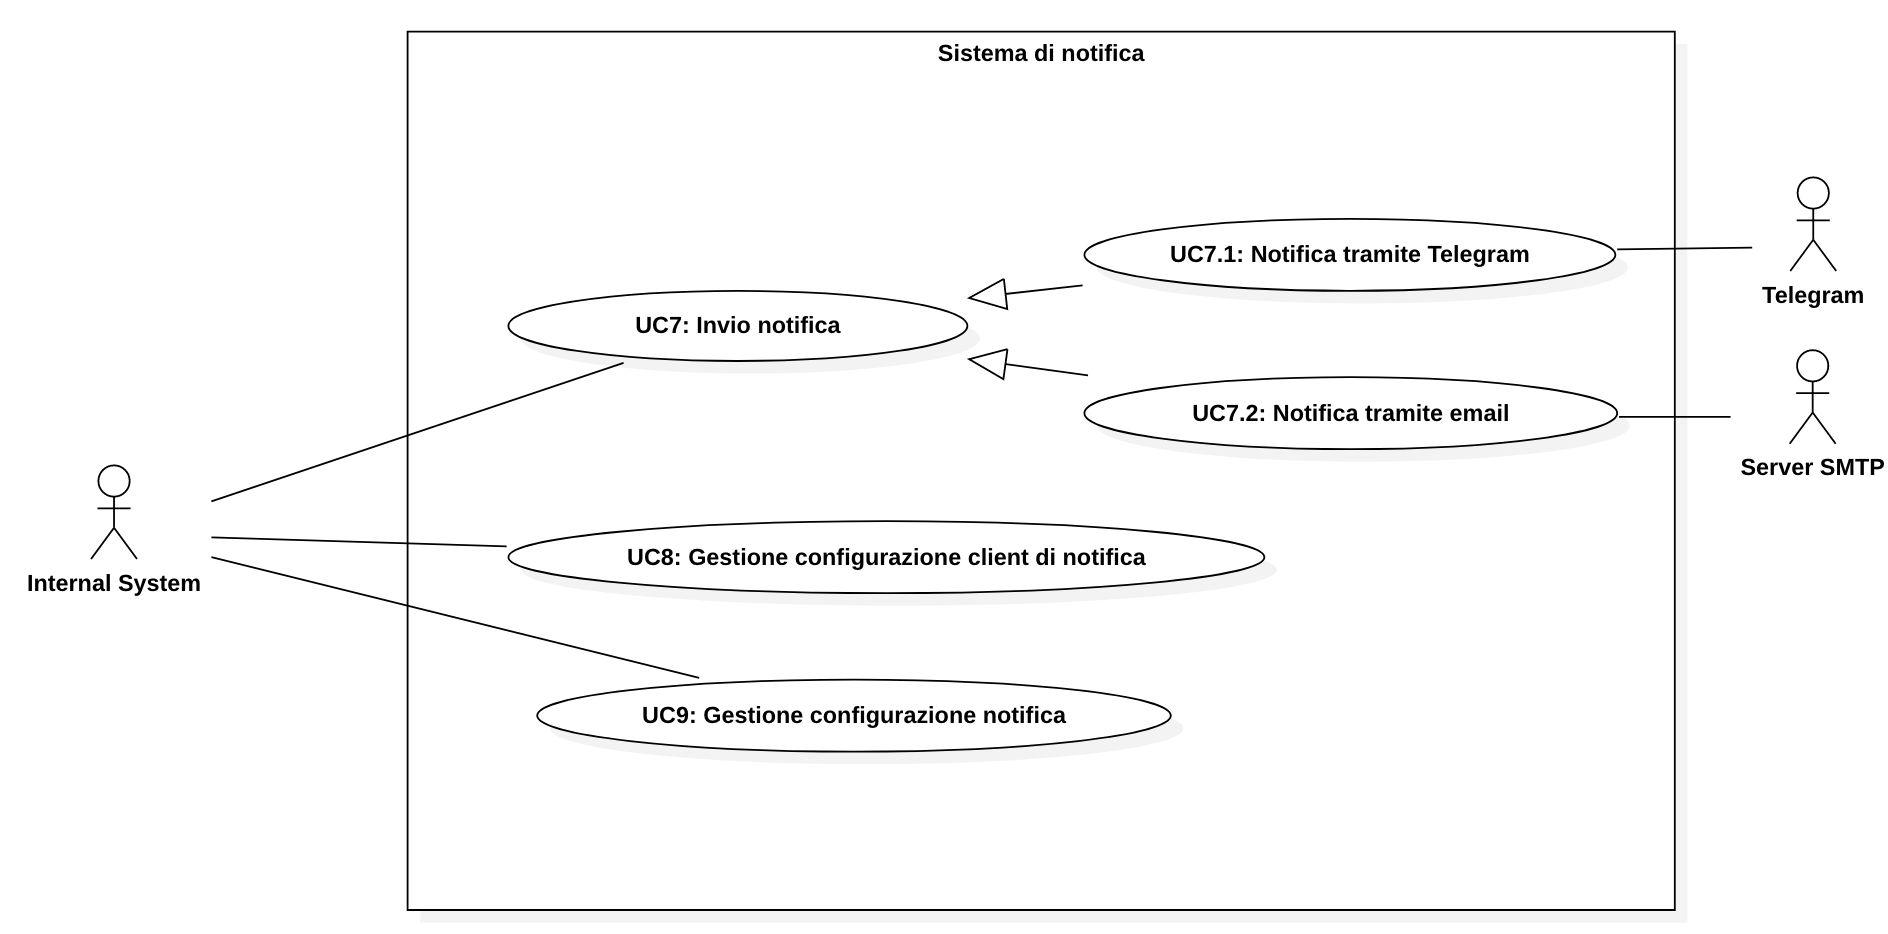
\includegraphics[keepaspectratio = true, width=15cm]{immagini/uc/5.png}
		\captionof{figure}{Use Case sistema di notifica}
\end{center}
\subsubsection{UC7 - Invio notifica}
\begin{itemize}
	\item \textbf{attore primario}: Internal System;
	\item \textbf{descrizione}: il sistema deve notificare una potenziale violazione delle \gloxy{S.L.A.};
	\item \textbf{precondizione}: il sistema ha trovato una potenziale violazione delle \gloxy{S.L.A.};
	\item \textbf{postcondizione}: il sistema ha notificato chi di dovere della potenziale violazione;
	\item \textbf{scenario principale}: 
	\begin{enumerate}
		\item il sistema viene avvisato di una potenziale violazione;
		\item il sistema invia la notifica al responsabile.
	\end{enumerate}
\end{itemize}
\paragraph{UC7.1 -  Notifica tramite Telegram}
\begin{itemize}
	\item \textbf{attore primario}: Internal System;
	\item \textbf{descrizione}: il sistema deve notificare una potenziale violazione delle \gloxy{S.L.A.};
	\item \textbf{precondizione}: il sistema ha trovato una potenziale violazione delle \gloxy{S.L.A.} e il \gloxy{Customer} associato ha \gloxy{Telegram} come canale di notifica;
	\item \textbf{postcondizione}: il sistema ha notificato chi di dovere tramite \gloxy{Telegram}  della potenziale violazione;
	\item \textbf{scenario principale}: 
	\begin{enumerate}
		\item il sistema viene avvisato di una potenziale violazione;
		\item il sistema invia la notifica tramite \gloxy{Telegram} al responsabile.
	\end{enumerate}
\end{itemize}
\paragraph{UC7.2 -  Notifica tramite email}
\begin{itemize}
	\item \textbf{attore primario}: Internal System;
	\item \textbf{descrizione}: il sistema deve notificare una potenziale violazione delle \gloxy{S.L.A.};
	\item \textbf{precondizione}: il sistema ha trovato una potenziale violazione delle \gloxy{S.L.A.} e il \gloxy{Customer} associato ha Email come canale di notifica;
	\item \textbf{postcondizione}: il sistema ha notificato chi di dovere tramite Email  della potenziale violazione;
	\item \textbf{scenario principale}: 
	\begin{enumerate}
		\item il sistema viene avvisato di una potenziale violazione;
		\item il sistema invia la notifica tramite Email al responsabile.
	\end{enumerate}
\end{itemize}
\subsubsection{UC8 - Gestione configurazione client di notifica}
\begin{itemize}
	\item \textbf{attore primario}: Internal System;
	\item \textbf{descrizione}: il sistema deve rendere disponibile un mezzo di configurazione per i vari canali di notifica;
	\item \textbf{precondizione}: il sistema è pronto per leggere la propria configurazione;
	\item \textbf{postcondizione}: il sistema ha letto correttamente la configurazione per ogni canale di notifica;
	\item \textbf{scenario principale}: 
	\begin{enumerate}
		\item il sistema viene avviato;
		\item il sistema legge la configurazione di ogni canale di notifica (e.g. le credenziali per \gloxy{Telegram}).
	\end{enumerate}
\end{itemize}
\subsubsection{UC9 - Gestione configurazione notifica}

\begin{center}
	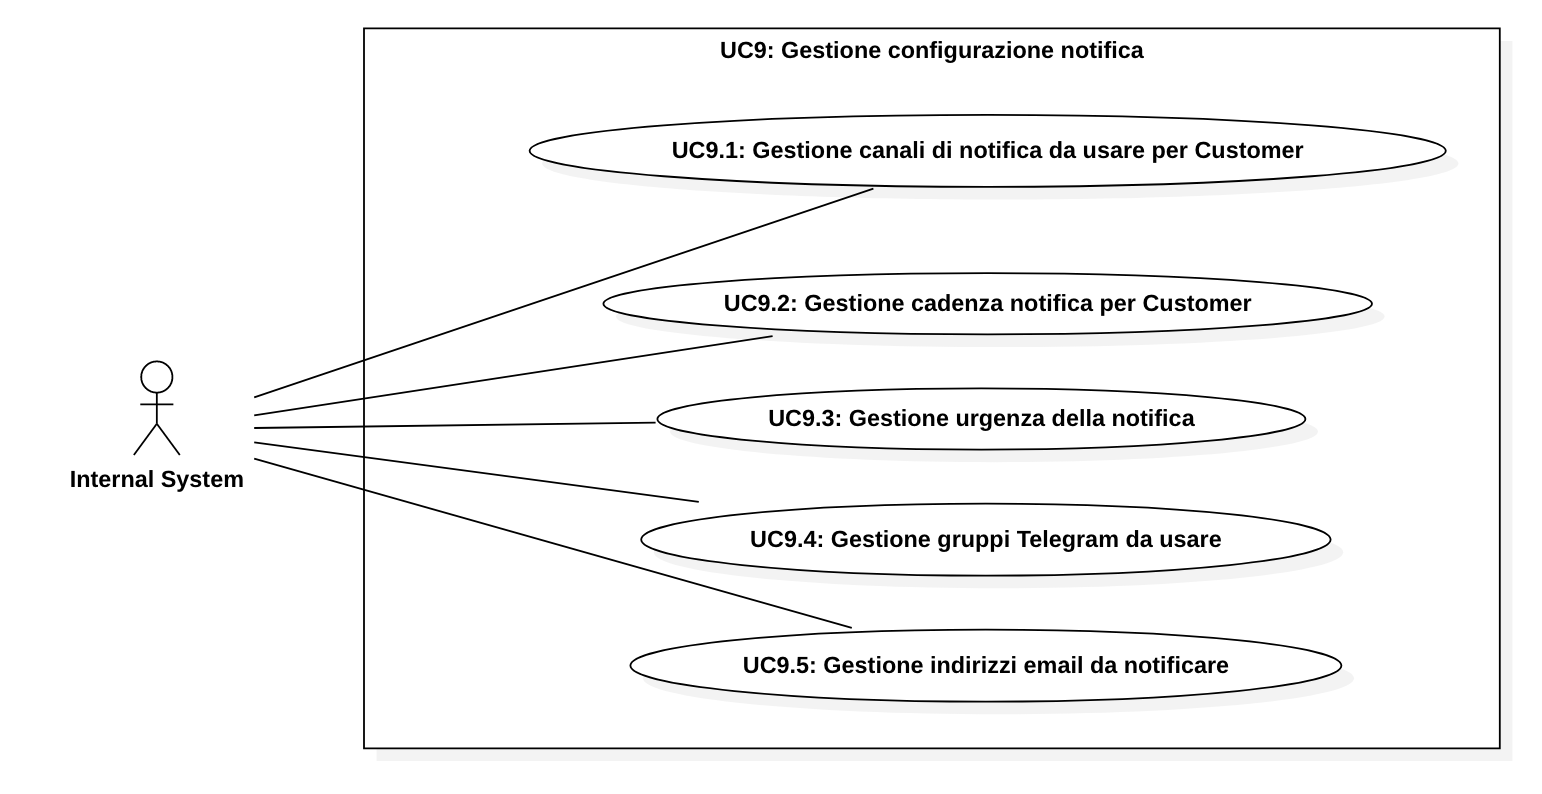
\includegraphics[keepaspectratio = true, width=15cm]{immagini/uc/6.png}
		\captionof{figure}{Sottocasi d'uso UC9}
\end{center}
\begin{itemize}
	\item \textbf{attore primario}: Internal System;
	\item \textbf{descrizione}: il sistema deve rendere disponibile un mezzo di configurazione per specificare il canale di notifica appropriato;
	\item \textbf{precondizione}: il sistema è pronto per leggere la propria configurazione;
	\item \textbf{postcondizione}: il sistema ha letto correttamente la configurazione per ogni \gloxy{Customer}; 
	\item \textbf{scenario principale}: 
	\begin{enumerate}
		\item il sistema viene avviato;
		\item il sistema legge la configurazione con le preferenze di notifica di ogni Customer.
	\end{enumerate}
\end{itemize}
\paragraph{UC9.1 -  Gestione canali di notifica per Customer}
\begin{itemize}
	\item \textbf{attore primario}: Internal System;
	\item \textbf{descrizione}: iIl sistema deve permettere di specificare che canali usare per la notifica di ogni \gloxy{Customer}; 
	\item \textbf{precondizione}: il sistema ha trovato una potenziale violazione delle \gloxy{S.L.A.} e il \gloxy{Customer} proprietario ha dei canali di notifica associati;
	\item \textbf{postcondizione}: il sistema ha notificato chi di dovere tramite i canali specificati della potenziale violazione;
	\item \textbf{scenario principale}: 
	\begin{enumerate}
		\item il sistema viene avvisato di una potenziale violazione.
		\item il sistema invia la notifica tramite i canali specificati avvisando di tale violazione.
	\end{enumerate}
\end{itemize}
\paragraph{UC9.2 -  Gestione cadenza di notifica per Customer}
\begin{itemize}
	\item \textbf{attore primario}: Internal System;
	\item \textbf{descrizione}: iIl sistema deve permettere di specificare che cadenza usare per la notifica di ogni \gloxy{Customer}; 
	\item \textbf{precondizione}: il sistema ha trovato una potenziale violazione delle \gloxy{S.L.A.} e il \gloxy{Customer} proprietario ha una cadenza di notifica associata;
	\item \textbf{postcondizione}: il sistema ha verificato se la cadenza è valida e in caso inviato la notifica;
	\item \textbf{scenario principale}: 
	\begin{enumerate}
		\item il sistema viene avvisato di una potenziale violazione;
		\item il sistema verifica se la cadenza è avvalorata, e se lo è invia la notifica di tale violazione.
	\end{enumerate}
\end{itemize}
\paragraph{UC9.3 -  Gestione urgenza di notifica per Customer}
\begin{itemize}
	\item \textbf{attore primario}: Internal System;
	\item \textbf{descrizione}: iIl sistema deve permettere di specificare che urgenza usare per la notifica di ogni \gloxy{Customer}; 
	\item \textbf{precondizione}: il sistema ha trovato una potenziale violazione delle \gloxy{S.L.A.} e il \gloxy{Customer} proprietario ha un'urgenza associata;
	\item \textbf{postcondizione}: il sistema ha inviato la notifica con l'urgenza associata;
	\item \textbf{scenario principale}: 
	\begin{enumerate}
		\item il sistema viene avvisato di una potenziale violazione;
		\item il sistema invia la notifica di violazione con l'urgenza associata a quel Customer.
	\end{enumerate}
\end{itemize}
\paragraph{UC9.4 -  Gestione gruppi telegram da usare}
\begin{itemize}
	\item \textbf{attore primario}: Internal System;
	\item \textbf{descrizione}: il sistema deve permettere di specificare che gruppi \gloxy{Telegram} usare per la notifica di ogni \gloxy{Customer}; 
	\item \textbf{precondizione}: il sistema ha trovato una potenziale violazione delle \gloxy{S.L.A.} e il \gloxy{Customer} proprietario ha dei gruppi \gloxy{Telegram} associati;
	\item \textbf{postcondizione}: il sistema ha inviato la notifica ai gruppi specificati;
	\item \textbf{scenario principale}: 
	\begin{enumerate}
		\item il sistema viene avvisato di una potenziale violazione;
		\item il sistema invia la notifica di violazione ai gruppi specificati.
	\end{enumerate}
\end{itemize}
\paragraph{UC9.5 -  Gestione indirizzi email da notificare}
\begin{itemize}
	\item \textbf{attore primario}: Internal System;
	\item \textbf{descrizione}: iIl sistema deve permettere di specificare che indirizzi email usare per la notifica di ogni \gloxy{Customer}; 
	\item \textbf{precondizione}: il sistema ha trovato una potenziale violazione delle \gloxy{S.L.A.} e il \gloxy{Customer} proprietario ha degli indirizzi email associati;
	\item \textbf{postcondizione}: il sistema ha inviato la notifica agli indirizzi email specificati;
	\item \textbf{scenario principale}: 
	\begin{enumerate}
		\item il sistema viene avvisato di una potenziale violazione;
		\item il sistema invia la notifica di violazione agli indirizzi specificati.
	\end{enumerate}
\end{itemize}

\subsection{Sistema di pubblicazione}
Gli use case identificati per questo sistema possono essere riassunti mediale il seguente diagramma UML:
\begin{center}
	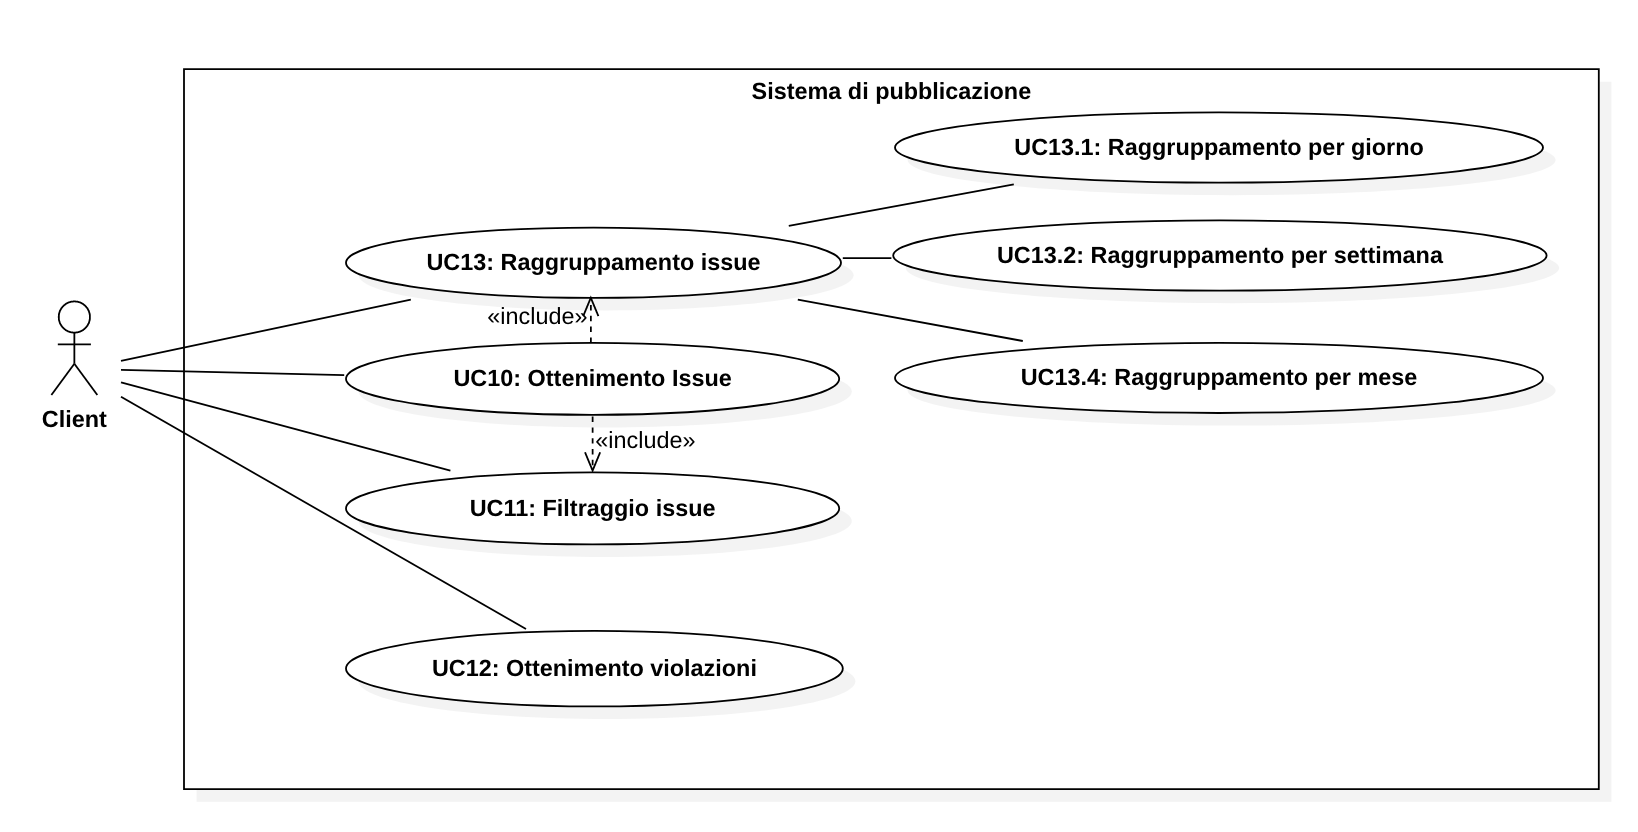
\includegraphics[keepaspectratio = true, width=15cm]{immagini/uc/7.png}
		\captionof{figure}{Use Case sistema di notifica}
\end{center}
\subsubsection{UC10 - Ottenimento issue}
\begin{itemize}
	\item \textbf{attore primario}: Client;
	\item \textbf{descrizione}: il sistema deve permettere ad un client di ottenere le \gloxy{issue};
	\item \textbf{precondizione}: il sistema è pronto per ricevere richieste;
	\item \textbf{postcondizione}: il client riceve le \gloxy{issue} richieste;
	\item \textbf{scenario principale}: 
	\begin{enumerate}
		\item il client invia una richiesta di ottenimento \gloxy{issue};
		\item il server risponde con la lista delle \gloxy{issue} richieste.
	\end{enumerate}
\end{itemize}
\subsubsection{UC11 - Filtraggio issue}
\begin{center}
	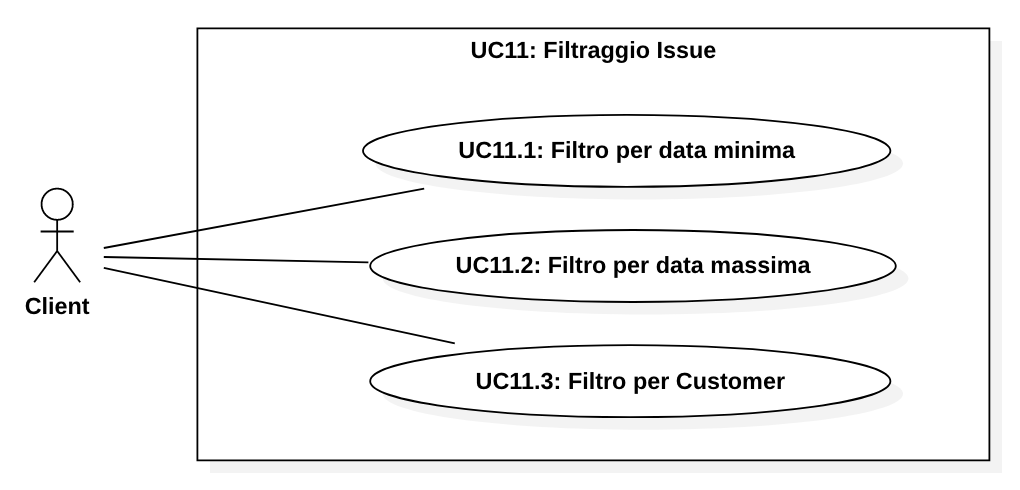
\includegraphics[keepaspectratio = true, width=15cm]{immagini/uc/8.png}
		\captionof{figure}{Sottocasi d'uso UC11}
\end{center}
\begin{itemize}
	\item \textbf{attore primario}: Client;
	\item \textbf{descrizione}: il client vuole ottenere le \gloxy{issue} filtrate rispetto alcuni criteri;
	\item \textbf{precondizione}: il sistema è pronto per ricevere richieste;
	\item \textbf{postcondizione}:  il client riceve le \gloxy{issue} filtrate rispetto ai parametri inviati;
	\item \textbf{scenario principale}: 
	\begin{enumerate}
		\item il client invia una richiesta di ottenimento \gloxy{issue};
		\item il server risponde con la lista delle \gloxy{issue} richieste filtrare rispetto ai parametri inviati.
	\end{enumerate}
\end{itemize}
\paragraph{UC11.1 - Filtro per data minima}
\begin{itemize}
	\item \textbf{attore primario}: Client;
	\item \textbf{descrizione}: iIl sistema deve permettere di specificare la data minima per il filtraggio delle \gloxy{issue};
	\item \textbf{precondizione}:  il sistema è pronto per ricevere richieste;
	\item \textbf{postcondizione}: il client riceve le \gloxy{issue} filtrate rispetto alla data di apertura (successiva alla data specificata nella richiesta);
	\item \textbf{scenario principale}: 
	\begin{enumerate}
		\item  il client invia una richiesta di ottenimento \gloxy{issue} specificando una data di apertura minima;
		\item  il server risponde con la lista delle \gloxy{issue} richieste filtrate rispetto alla data di apertura (maggiore di quella richiesta).
	\end{enumerate}
\end{itemize}
\paragraph{UC11.2 - Filtro per data massima}
\begin{itemize}
	\item \textbf{attore primario}: Client;
	\item \textbf{descrizione}: iIl sistema deve permettere di specificare la data massima per il filtraggio delle \gloxy{issue};
	\item \textbf{precondizione}:  il sistema è pronto per ricevere richieste;
	\item \textbf{postcondizione}: il client riceve le \gloxy{issue} filtrate rispetto alla data di apertura (precedente alla data specificata nella richiesta);
	\item \textbf{scenario principale}: 
	\begin{enumerate}
		\item  il client invia una richiesta di ottenimento \gloxy{issue} specificando una data di apertura massima;
		\item  il server risponde con la lista delle \gloxy{issue} richieste filtrate rispetto alla data di apertura (minore di quella richiesta).
	\end{enumerate}
\end{itemize}
\paragraph{UC11.3 - Filtro per Customer}
\begin{itemize}
	\item \textbf{attore primario}: Client;
	\item \textbf{descrizione}: iIl sistema deve permettere di specificare il \gloxy{Customer} di cui si vuole ottenere le \gloxy{issue};
	\item \textbf{precondizione}:  il sistema è pronto per ricevere richieste;
	\item \textbf{postcondizione}: il client riceve le \gloxy{issue} filtrate rispetto al \gloxy{Customer} richiesto (precedente alla data specificata nella richiesta);
	\item \textbf{scenario principale}: 
	\begin{enumerate}
		\item  il client invia una richiesta di ottenimento \gloxy{issue} specificando un \gloxy{Customer}; 
		\item  il server risponde con la lista delle \gloxy{issue} richieste filtrate rispetto al \gloxy{Customer} richiesto.
	\end{enumerate}
\end{itemize}

\subsubsection{UC12 - Ottenimento violazioni}
\begin{itemize}
	\item \textbf{attore primario}: Client;
	\item \textbf{descrizione}: il client vuole ottenere una lista di violazioni;
	\item \textbf{precondizione}:  il sistema è pronto per ricevere richieste;
	\item \textbf{postcondizione}: il client riceve la lista delle violazioni richiesta;
	\item \textbf{scenario principale}: 
	\begin{enumerate}
		\item il client invia una richiesta di ottenimento delle violazioni;
		\item il server risponde con la lista delle violazioni richieste.
	\end{enumerate}
\end{itemize}
\subsubsection{UC13 - Raggruppamento issue}
\begin{itemize}
	\item \textbf{attore primario}: Client;
	\item \textbf{descrizione}: il client vuole ottenere una lista di \gloxy{issue} raggruppate secondo un certo criterio;
	\item \textbf{precondizione}:  il sistema è pronto per ricevere richieste;
	\item \textbf{postcondizione}: il client riceve la lista delle \gloxy{issue} raggruppata come richiesta;
	\item \textbf{scenario principale}: 
	\begin{enumerate}
		\item il client invia una richiesta di ottenimento delle \gloxy{issue} specificando un criterio di raggruppamento;
		\item il server risponde con la lista delle \gloxy{issue} raggruppata come richiesta.
	\end{enumerate}
\end{itemize}
\paragraph{UC13.1 - Raggruppamento issue per giorno}
\begin{itemize}
	\item \textbf{attore primario}: Client;
	\item \textbf{descrizione}: il client vuole ottenere una lista di \gloxy{issue} raggruppate per giorno di apertura;
	\item \textbf{precondizione}:  il sistema è pronto per ricevere richieste;
	\item \textbf{postcondizione}: il client riceve la lista delle \gloxy{issue} raggruppata come richiesta;
	\item \textbf{scenario principale}: 
	\begin{enumerate}
		\item il client invia una richiesta di ottenimento delle \gloxy{issue} richiedendo di raggrupparle per giorno;
		\item il server risponde con la lista delle \gloxy{issue} raggruppata per giorno.
	\end{enumerate}
\end{itemize}
\paragraph{UC13.1 - Raggruppamento issue per settimana}
\begin{itemize}
	\item \textbf{attore primario}: Client;
	\item \textbf{descrizione}: il client vuole ottenere una lista di \gloxy{issue} raggruppate per settimana di apertura;
	\item \textbf{precondizione}:  il sistema è pronto per ricevere richieste;
	\item \textbf{postcondizione}: il client riceve la lista delle \gloxy{issue} raggruppata come richiesta;
	\item \textbf{scenario principale}: 
	\begin{enumerate}
		\item il client invia una richiesta di ottenimento delle \gloxy{issue} richiedendo di raggrupparle per settimana;
		\item il server risponde con la lista delle \gloxy{issue} raggruppata per settimana.
	\end{enumerate}
\end{itemize}
\paragraph{UC13.1 - Raggruppamento issue per mese}
\begin{itemize}
	\item \textbf{attore primario}: Client;
	\item \textbf{descrizione}: il client vuole ottenere una lista di \gloxy{issue} raggruppate per mese di apertura;
	\item \textbf{precondizione}:  il sistema è pronto per ricevere richieste;
	\item \textbf{postcondizione}: il client riceve la lista delle \gloxy{issue} raggruppata come richiesta;
	\item \textbf{scenario principale}: 
	\begin{enumerate}
		\item il client invia una richiesta di ottenimento delle \gloxy{issue} richiedendo di raggrupparle per mese;
		\item il server risponde con la lista delle \gloxy{issue} raggruppata per mese.
	\end{enumerate}
\end{itemize}















\section{Tracciamento requisiti}
In questa sezione, vengono riportati i requisiti del progetto, classificati per obbligatorietà. Ciascun requisito possiede un codice identificativo, il cui formalismo viene riportato di seguito:
\begin{center}
	\textbf{R<NumeroRequisito>.<NumeroSottoRequisito>-<Classificazione>}
\end{center}
La classificazione andrà a specificare l'obbligatorietà del requisito, e potrà essere indicata tramite una delle due seguenti sigle:
\begin{itemize}
	\item \textbf{O}: requisito obbligatorio
	\item \textbf{D}: requisito desiderabile
\end{itemize}

\subsection{Requisiti}

\begin{center}
	\rowcolors{2}{lightest-grayest}{white}
	\begin{longtable}{|p{3cm}|p{8cm}|p{3cm}|}
		\hline
		\rowcolor{lighter-grayer}
		\textbf{Requisito} & \textbf{Descrizione} \\ \hline
		R1-O & L'engine deve interfacciarsi con \gloxy{Redmine} per l'ottenimento delle informazioni riguardanti a \gloxy{Customers}  e Issues \\ \hline
		R2-O & L'engine deve potersi autenticare presso \gloxy{Redmine} tramite \gloxy{API key} \\ \hline
		R3-O & L'engine deve permettere una configurazione dinamica delle \gloxy{S.L.A.} per ogni \gloxy{Customer} \\ \hline
		R3.1-O & L'engine deve permettere una configurazione dinamica della durata massima di presa in carico per i ticket di ogni \gloxy{Customer} \\ \hline
		R3.2-O & L'engine deve permettere una configurazione dinamica della durata massima di risoluzione per i ticket di ogni \gloxy{Customer} \\ \hline
		R4-O & L'engine deve rendere disponibili canali di notifica per la segnalazione di violazioni delle \gloxy{S.L.A.} \\ \hline
		R4.1-D & L'engine deve rendere disponibile Email come canale per la segnalazione di violazioni delle \gloxy{S.L.A.} \\ \hline
		R4.1-D & L'engine deve rendere disponibile la possibilità di specificare un'email come canale per la segnalazione di violazioni delle \gloxy{S.L.A.} customizzabile per ogni \gloxy{Customer}  \\ \hline
		R4.2-D & L'engine deve rendere disponibile \gloxy{Telegram}  come canale per la segnalazione di violazioni delle \gloxy{S.L.A.} \\ \hline
		R4.3-D & L'engine deve rendere disponibile  la possibilità di specificare un gruppo \gloxy{Telegram}  come canale per la segnalazione di violazioni delle \gloxy{S.L.A.} customizzabile per ogni \gloxy{Customer}  \\ \hline
		R5-O & L'engine deve notificare al responsabile designato potenziali violazioni delle \gloxy{S.L.A.} \\ \hline
		R6-D & L'engine deve permettere di configurare i vari canali di notifica definiti per la segnalazione di violazioni (e.g. le credenziali per la connessione SMTP)\\ \hline
		R7-O & L'engine deve mettere a disposizione un'\gloxy{API} per la pubblicazione dei dati\\ \hline
		R7.1-D & L'engine deve mettere a disposizione un'\gloxy{API} per la pubblicazione delle issue\\ \hline
		R7.2-D & L'engine deve mettere a disposizione un'\gloxy{API} per la pubblicazione delle violazioni\\ \hline
		R8-D & L'engine deve prevedere un modo per rendere personalizzabile l'intervallo di aggiornamento da \gloxy{Redmine}\\ \hline
		R9-O & L'engine deve permettere una facile migrazione a un sistema di gestione di Ticket diverso da \gloxy{Redmine}\\ \hline
		R10-O & L'engine deve prevedere degli \gloxy{S.L.A.} di default\\ \hline
		R11-O & L'engine deve prevedere la possibilità di categorizzare le violazioni per  “info”, “warning”, “urgent” ed “escalation”\\ \hline
		R12-O & L'engine deve prevedere la possibilità di aggiornare su richiesta i dati su \gloxy{Redmine} tramite \gloxy{API}\\ \hline
		R13-O & L'engine deve prevedere un servizio per esportare dei dati in qualche formato\\ \hline
		R14-O & L'engine deve prevedere un modo per memorizzare localmente gli aggiornamenti ricevuti da \gloxy{Redmine} \\ \hline
		R15-O & L'engine deve prevedere un modo per andare periodicamente a scaricare gli aggiornamenti da \gloxy{Redmine}\\ \hline
		
		\rowcolor{light-grayer}
		\multicolumn{2}{|l|}{\textbf{API}} \\ \hline
		R16-D & L'\gloxy{API} deve permettere il filtraggio tramite data minima dove possibile\\ \hline
		R17-D & L'\gloxy{API} deve permettere il filtraggio tramite data massima dove possibile\\ \hline
		R18-D & L'\gloxy{API} deve permettere di raggruppare i dati richiesti dove possibile\\ \hline
		R18.1-D & L'\gloxy{API} deve permettere di raggruppare i dati richiesti per giorno dove possibile\\ \hline
		R18.2-D & L'\gloxy{API} deve permettere di raggruppare i dati richiesti per settimana dove possibile\\ \hline
		R18.3-D & L'\gloxy{API} deve permettere di raggruppare i dati richiesti per mese dove possibile\\ \hline
		
		
		R19-D & L'\gloxy{API} deve fornire la possibilità di sapere per ogni \gloxy{Customer} quanti \gloxy{Ticket} ha avuto    \\ \hline
		R20-D & L'\gloxy{API} deve fornire la possibilità di sapere per ogni \gloxy{Customer} quante violazioni ha subito   \\ \hline
		R21-D & L'\gloxy{API} deve fornire la possibilità di sapere per ogni \gloxy{Ticket} quanto tempo in carico è stato a Euronovate e quanto al cliente\\ \hline
		R22-D & L'\gloxy{API} deve fornire la possibilità di ottenere il tempo medio di risoluzione di ticket\\ \hline
		R23-D & L'\gloxy{API} deve fornire la possibilità di ottenere il tempo medio di presa in carico di ticket\\ \hline
		
		
		
		% R-O & L'\gloxy{API}    \\ \hline
		
		\rowcolor{white}
		\caption{Elenco requisiti}
	\end{longtable}
\end{center}








